

\section{Auswertung}
Zunächst wird der Acrylblock ausgemessen.
Der Acrylblock hat eine Tiefe von 8\,cm.\\
Die Abstände zu den einzelnen Fehlstellungen sind in Tabelle \ref{tab:ausmessung} aufgelistet.
\begin{table}[H]
  \centering
  \caption{Ausmessung der Acrylblocks}
  \label{tab:ausmessung}
  \begin{tabular}{c c c c}
    \toprule
    {Fehlstelle} & {$s_{oben} / \mathrm{cm}$} & {$s_{unten} / \mathrm{cm}$} & {$d_{Fehlstelle}$ / cm}\\
    \midrule
    1  & 1,9 & 5,9 & 0,2\\
    2  & 1,7 & 6,1 & 0,2\\
    3  & 6,1 & 1,3 & 0,6\\
    4  & 5,4 & 2,1 & 0,5\\
    5  & 4,6 & 3,0 & 0,4\\
    6  & 3,9 & 3,9 & 0,2\\
    7  & 3,1 & 4,6 & 0,3\\
    8  & 2,3 & 5,4 & 0,3\\
    9  & 1,4 & 6,3 & 0,3\\
    10 & 0,7 & 7,1 & 0,2\\
    11 & 5,5 & 1,5 & 1,0\\
    \bottomrule
  \end{tabular}
\end{table}

\subsection{Ausmessung des Acrylblocks mit dem A-Scan}
Nun wird der Acrylblock mit Hilfe des A-Scans ausgemessen.
Die Werte sind in Tabelle \ref{tab:A} zu finden.
Dabei wurde die Schallgeschwindigkeit von 2730\,$\mathrm{ms^{-1}}$ \cite{schall} schon berücksichtigt.
Die prozentualen Abweichungen ergeben sich durch einen Vergleich der Werte,
die in Tabelle \ref{tab:ausmessung} angegeben sind.
Die Formel lautet:
\begin{equation}
  p = \left|\frac{s_{\symup{mess}}-s_{\symup{theo}}}{s_{\symup{theo}}}\right|
  \label{eqn:abweichung}
\end{equation}
\begin{table}
  \centering
  \caption{Ausmessung mit dem A-Scan}
  \label{tab:A}
  \begin{tabular}{c c c c c c}
    \toprule
    {Ultraschallsonde} & {Fehlstelle} & {s$_{oben}$ / mm} & {$s_{unten}$ / mm} &
    {oben / $\%$} & {unten / $\%$}\\
    \midrule
    blau (1\,MHz) & 1  & 19 & 59 & 0    & 0   \\
         & 2  & 19 & 59 & 11,8 & 3,3 \\
         & 3  & 61 & 12 & 0    & 7,7 \\
         & 4  & 53 & 21 & 1,9  & 0   \\
         & 5  & 43 & 29 & 8,5  & 3,3 \\
         & 6  & 38 & 38 & 2,6  & 2,6 \\
         & 7  & 30 & 46 & 3,2  & 0   \\
         & 8  & 22 & 54 & 4,3  & 0   \\
         & 9  & 15 & 62 & 7,1  & 1,6 \\
         & 10 & 6  &    & 14,3 &     \\
         & 11 &    & 14 &      & 6,7 \\
    rot (2\,MHz)  & 1  & 16 & 57 & 15,8 & 3,4 \\
         & 2  & 18 & 59 & 5,9  & 3,3 \\
    \bottomrule
  \end{tabular}
\end{table}
Die Fehlstellen 1 und 2 wurden mit zwei Unterschiedlichen Sonden ausgemessen.
Die höhere Frequenz der roten Sonde sorgt für eine bessere Darstellung der nah aneinander liegenden Fehlstellen.
Die aufgenommenen Bilder des A-Scans sind für die beiden Sonden in Abbildung \ref{fig:boben}, \ref{fig:bunten}, \ref{fig:roben}
und \ref{fig:runten} zu sehen.
\begin{figure}[H]
\centering
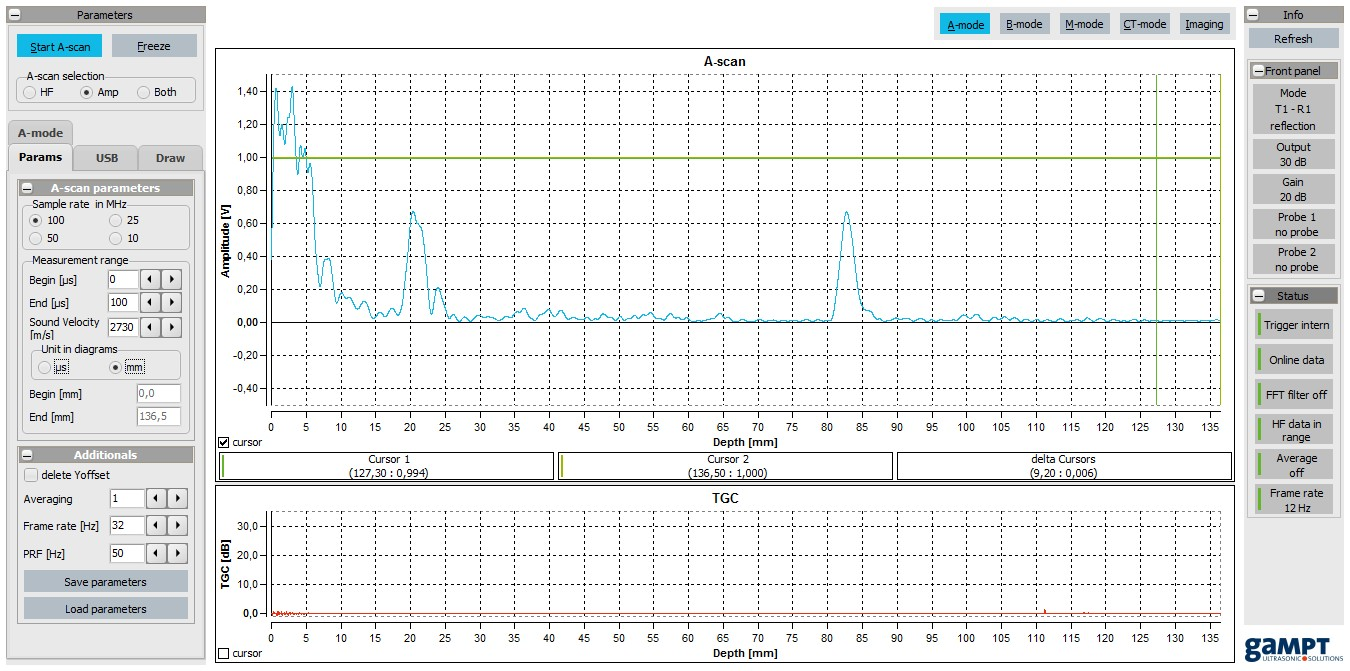
\includegraphics[width=\textwidth]{12a.jpg}
\caption{Messung der Fehlstellen 1 und 2 mit der blauen Sonde von oben}
\label{fig:boben}
\end{figure}

\begin{figure}[H]
\centering
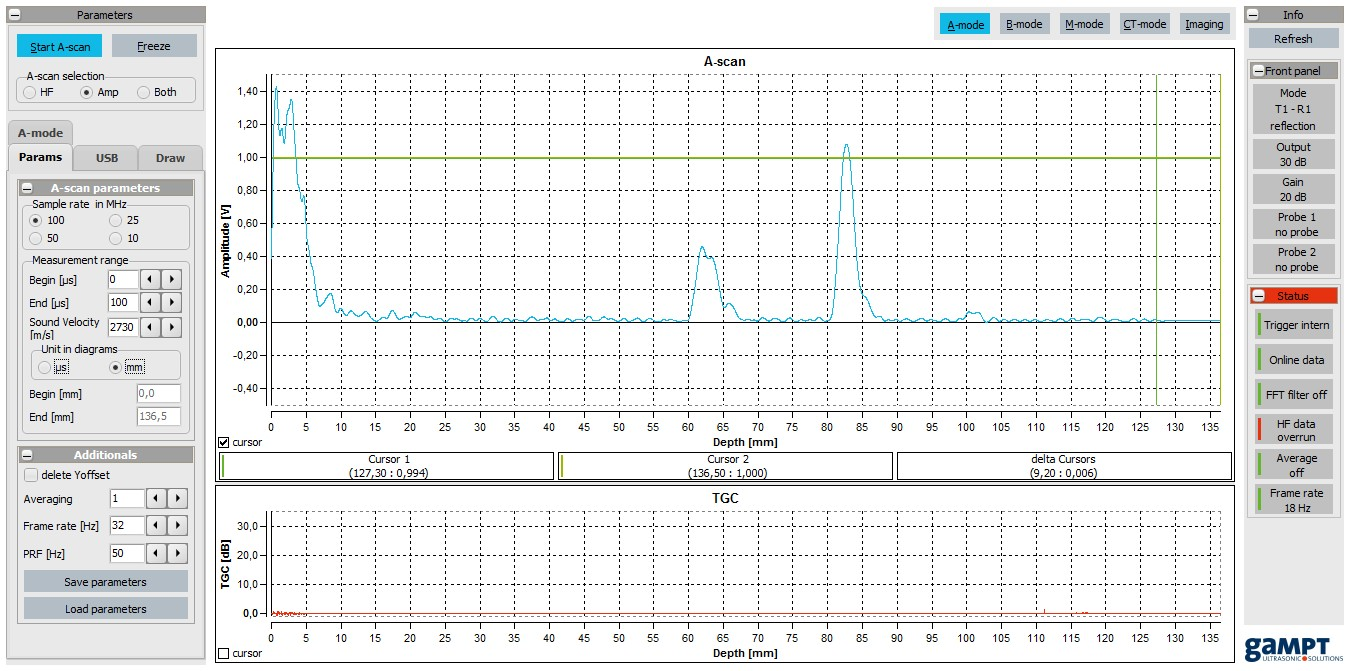
\includegraphics[width=\textwidth]{12blauunten.jpg}
\caption{Messung der Fehlstellen 1 und 2 mit der blauen Sonde von unten}
\label{fig:bunten}
\end{figure}

\begin{figure}[H]
\centering
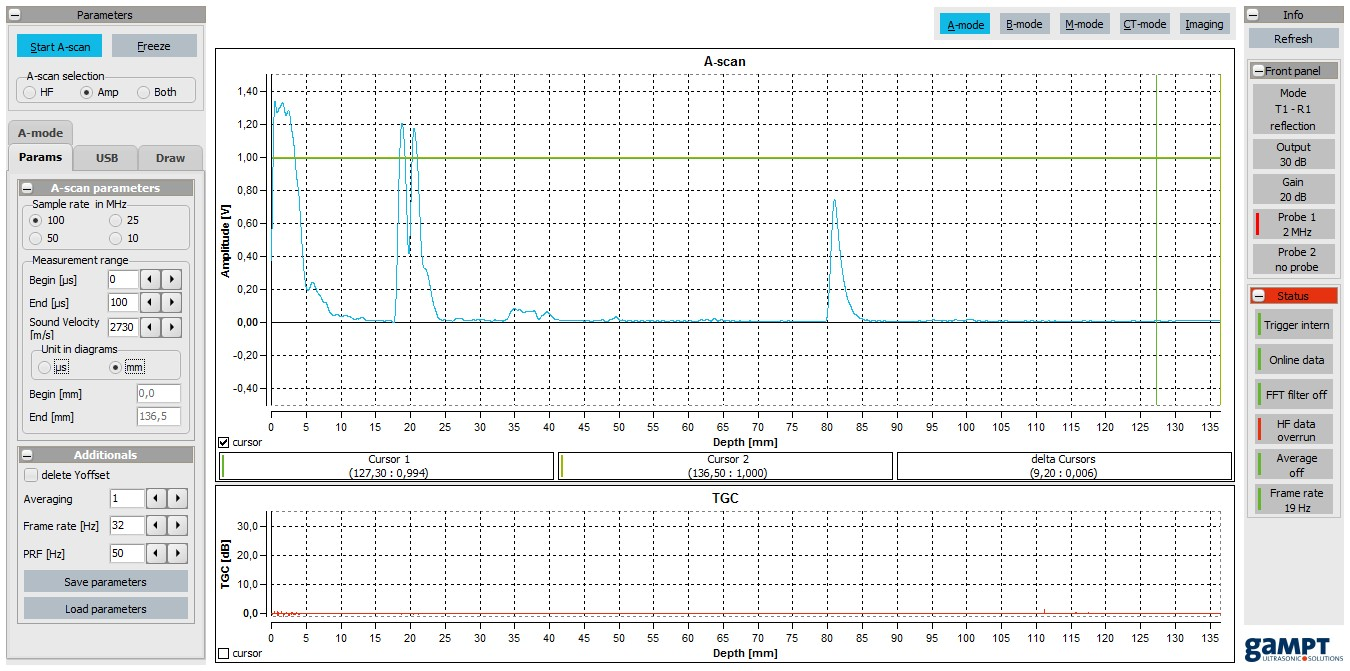
\includegraphics[width=\textwidth]{12rotoben.jpg}
\caption{Messung der Fehlstellen 1 und 2 mit der roten Sonde von oben}
\label{fig:roben}
\end{figure}

\begin{figure}[H]
\centering
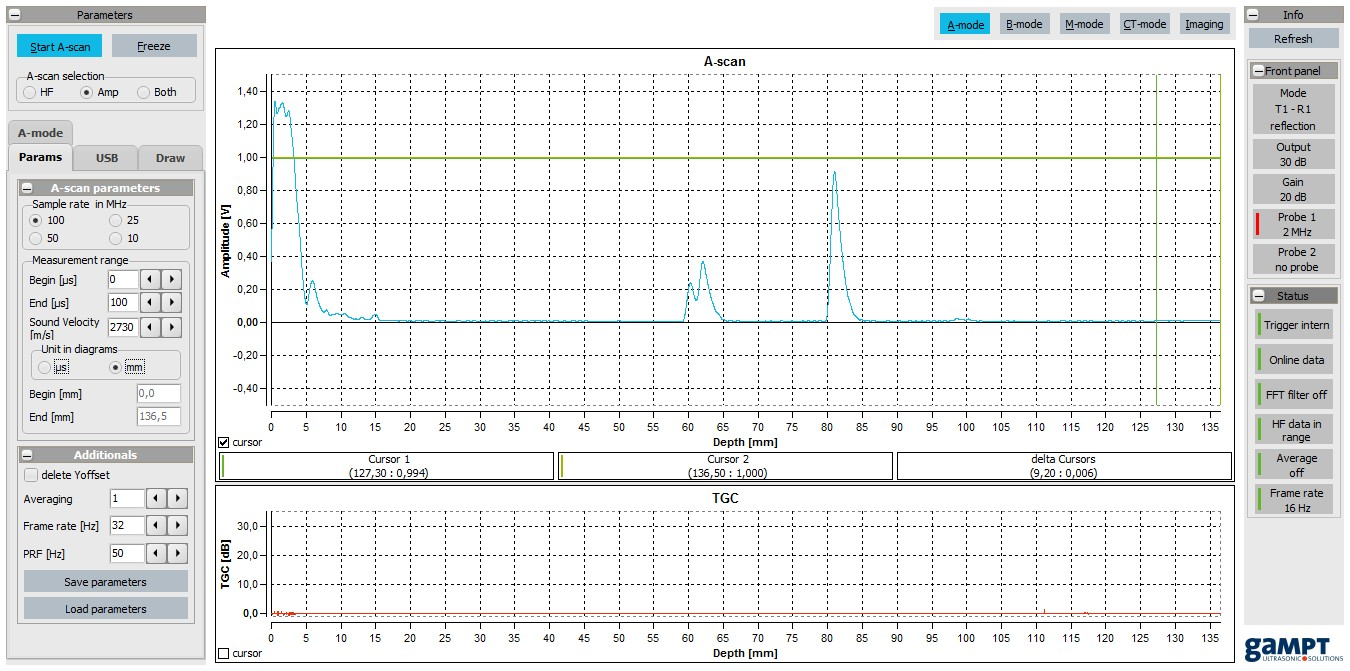
\includegraphics[width=\textwidth]{12rotunten.jpg}
\caption{Messung der Fehlstellen 1 und 2 mit der roten Sonde von unten}
\label{fig:runten}
\end{figure}

\subsection{Ausmessung des Acrylblocks mit dem B-Scan}
In den Abbildungen \ref{fig:boben} und \ref{fig:bunten} sind die gemessenen B-Scans zu sehen.
Aus diesen Abbildungen werden die Werte in Tabelle \ref{tab:B} entnommen.
Dabei war darauf zu achten, dass von den Werten die Wasserschicht abgezogen wird.
Diese wird ebenfalls aus den Abbildungen entnommen und beträgt 3,45\,mm.
\begin{figure}
\centering
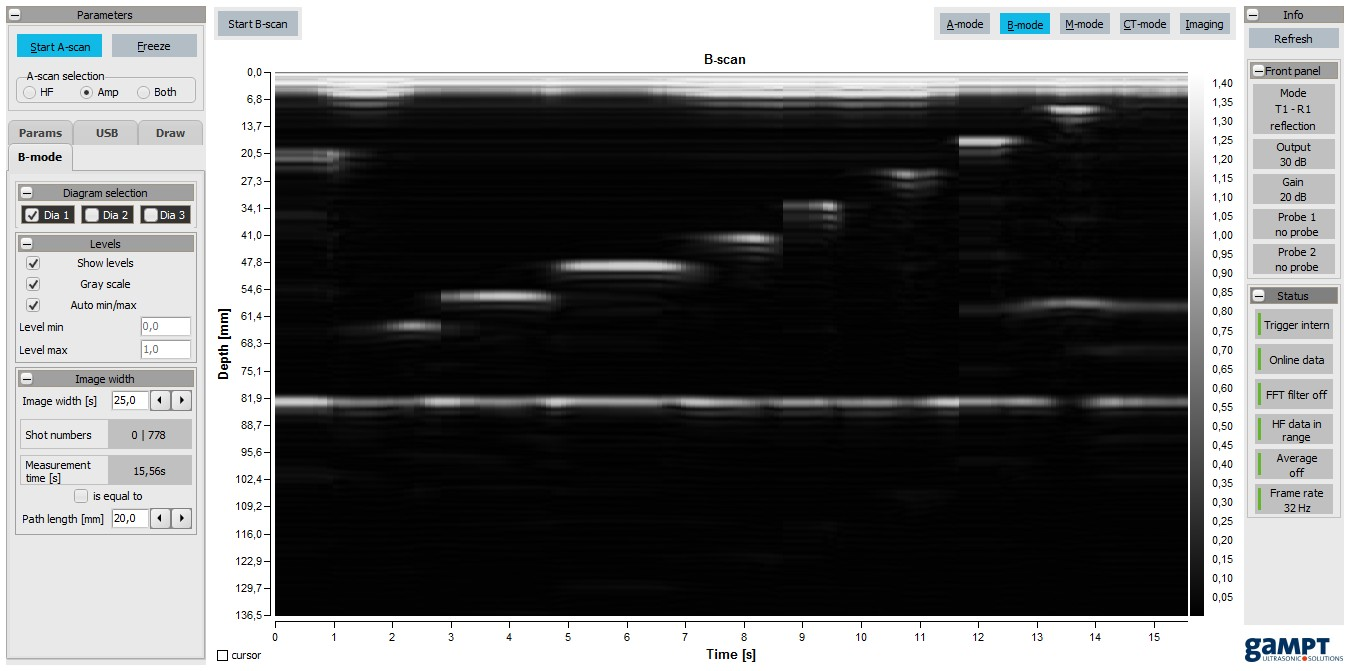
\includegraphics[width=\textwidth]{Bscanoben.jpg}
\caption{B-Scan des Acrylblocks von oben}
\label{fig:boben}
\end{figure}

\begin{figure}
\centering
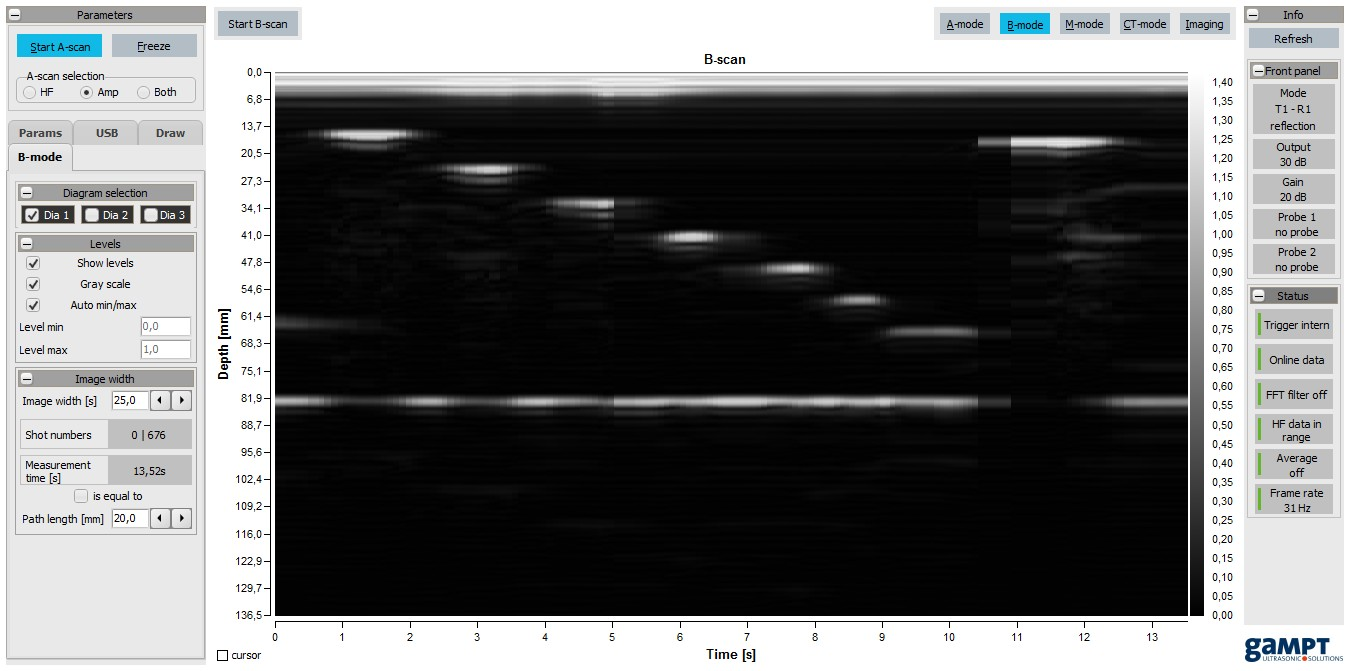
\includegraphics[width=\textwidth]{bscanunten.jpg}
\caption{B-Scan des Acrylblocks von unten}
\label{fig:bunten}
\end{figure}

\begin{table}
  \centering
  \caption{Ausmessung mit dem B-Scan}
  \label{tab:B}
  \begin{tabular}{c c c c c c}
    \toprule
     {Fehlstelle} & {s$_{oben}$ / mm} & {$s_{unten}$ / mm} &
    {oben / $\%$} & {unten / $\%$}\\
    \midrule
         1  & 17,74 &       & 6,6 &    \\
         2  & 17,74 &       & 4,4 &  \\
         3  & 60,71 & 13,7  & 0,5 & 5,4 \\
         4  & 53,22 & 21,88 & 1,4 & 4,2 \\
         5  & 45,73 & 29,27 & 0,6 & 2,4 \\
         6  & 38,24 & 38,93 & 1,9 & 0,2 \\
         7  & 30,65 & 47,11 & 1,1 & 2,4 \\
         8  & 23,16 & 54,6  & 0,7 & 1,1 \\
         9  & 13,7  & 62,78 & 2,1 & 0,3 \\
         10 & 6,8   &       & 2,9 &     \\
         11 & 56,57 & 14,98 & 2,9 & 0,1 \\
    \bottomrule
  \end{tabular}
\end{table}
Die prozentuale Abweichung wurde mit Formel (\ref{eqn:abweichung}) bestimmt.

\subsection{Untersuchung eines Herzmodells}
Zunächst wird der Zylinder ausgemessen.
\begin{align*}
  d_{Wand}&=0,2\,\mathrm{cm} & d_{gefäß}= 4,71\, \mathrm{cm}\\
  &\Rightarrow d_{ges}= 4,51\,\mathrm{cm}
\end{align*}
Die mit Abbildung \ref{fig:herz} bestimmte Herzfrequenz beträgt 27\,bpm.
Das entspricht einer Frequenz von 450\,mHz.
Nun wird ein A-Scan durchgeführt.
Es werden die Störstellen bei ruhender Membran und gepumpter Membran aufgenommen.
\begin{align*}
  s_{r} &= 34\,\mathrm{mm}\\
  s_{p} &= 56\,\mathrm{mm}
\end{align*}
Das Herzzeitvolumen (HZV) berechnet sich mit der Formel
\begin{equation}
  HZV = (ESV-EDV)\cdot \nu
\end{equation}
Dabei ist ESV das endsystolische Volumen und EDV das enddiastolische Volumen .
Somit ergibt sich das HZV zu
\begin{align*}
  HZV &= \pi r^2(s_p -s_r) \nu\\
      &= \pi (2,255\cdot10^{-2})^2\cdot(56-34)10^{-3}\cdot 450\cdot10^{-3}\\
      &= 1,58\cdot10^{-5}\,\mathrm{\frac{m^3}{s}}
\end{align*}

\begin{figure}
  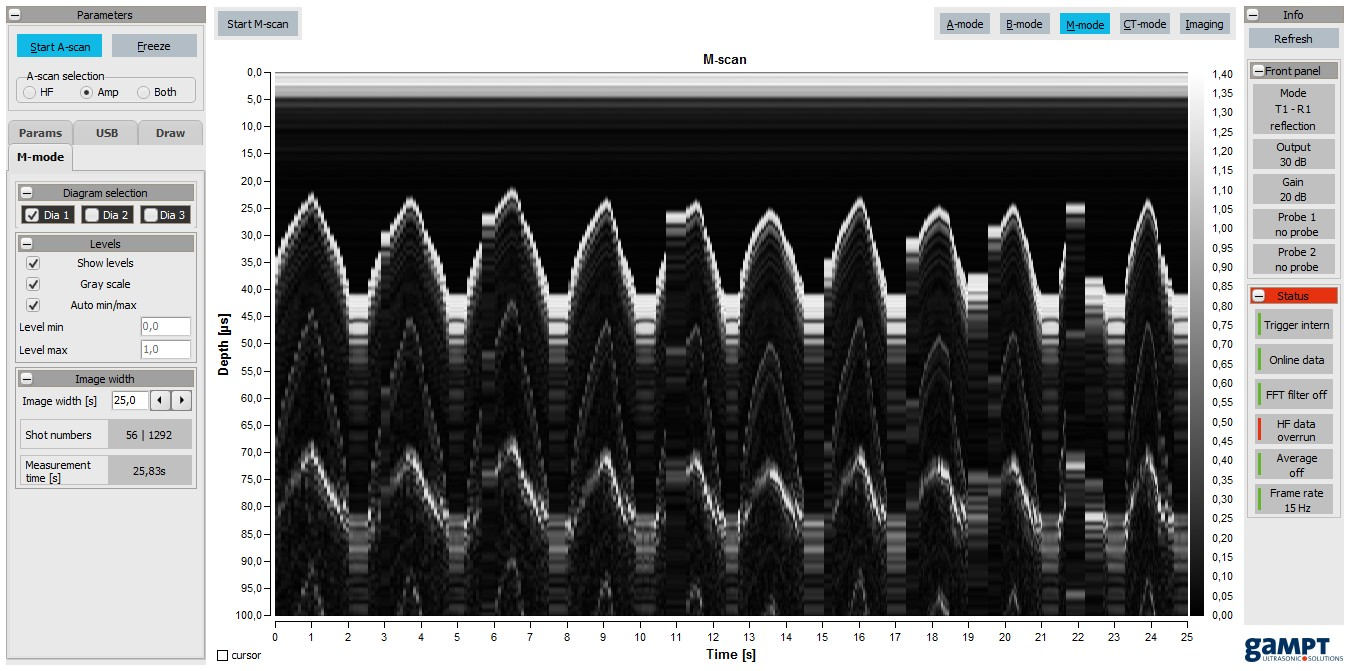
\includegraphics[width=\textwidth]{herz.jpg}
  \caption{Time-Motion Scan eines Herzmodells}
  \label{fig:herz}
\end{figure}

\section{Diskussion}

Die Abweichungen der mit dem A- und B-Scan bestimmten Werte sind im Vergleich zu den theoretischen Werten gering.
Dabei ist zu beachten, dass die theoretischen Werte mittels einer Schieblehre bestimmt wurden und somit ebenfalls fehlerbelastet sind.
Es ist zu erkennen, dass die Abweichungen beim B-Scan insgesamt geringer sind
und dies somit das genauere Verfahren ist.
Die Fehlerstellen 1, 2, 10  und 11 konnten nicht immer mit angegeben werden,
da aufgrund der unterschiedlich benutzten Sonden die Messung nicht möglich war.
Das liegt zum einen daran, dass niedrige Frequenzen eine höhere Wellenlänge besitzen
und somit enger aneinander liegende Störstellen nicht einzeln Messbar sind,
zum anderen daran, dass niedrige Frequenzen auch geringer in das Material eindringen.\\
Im letzten Teil des Versuchs wird die Herzfrequenz mit Hilfe der Abbildung \ref{fig:herz} bestimmt.
Somit ist zu beachten, dass es hier ebenfalls eine Fehlerbelastung gibt.
